\section{Experiments} \label{sec:experiments}


\subsection{Baseline Methods} \label{subsec:baseline}

In this section we will go through the experiments performed in order to get
our baseline results. While many different features can be used when performing
\gls{NLP}, we chose the same features, as was used in \cite{US}, since they
span several several of the different linguistic layers. The linguistic layers
are different areas which all serve to describe a certain text. An example this
could be the character level layer, which as the name implies, focuses on the
individual characters used in a specific text. Other examples of this, could
be the sentence layer, that focuses on the sentences of the text, and the meta
layer, that focuses on things such as publishing/delivery date, and file format.
The features available to pick from in this case are:

\begin{itemize}
    \item Word-N-grams,
    \item Character-N-grams,
    \item Word Frequencies (word-1-grams),
    \item \gls{POS}-tag-N-grams, and
    \item Special-Character-N-grams,
\end{itemize}

Where an N-gram describes the combinations of sequential elements of size n. In
the case where that element is characters, and n is 3, the string "hello" would
produce the character-3-grams "hel", "ell" and "llo". This also means that a
feature such as word frequencies can be considered word-1-grams.

\gls{POS} tags, refer to the grammatical class a certain words belongs to,
such as nouns and adjectives. In order to extract these we made use
of a POS-tag extractor, provided by \cite{polyglot}.

For all of these experiments a Danish third party corpus, provided by
\texttt{NLTK}\footnote{\url{http://www.nltk.org/index.html}}, was used as the
basis for all the feature extraction, as was done in \cite{US} as well. This
corpus consists of 22,476 sentences, and 563,358 words.

The actual implementation of both the \gls{SVM} and the Extended Delta method,
very closely resembles the implementation used in \cite{US}. There is however
a very big difference, with the actual application of the delta method.
Contrary to the scenario in \cite{US}, where PAN data was used, there isn't an
instance where we only have 1 text per author. As such the original version
of the delta method can be used. This is where, when given a new text $x$
supposedly written by an author $\alpha \in \mathcal{A}$, his texts $T_\alpha$
are extracted, and so is a set of texts no written by him $\overline{T}_alpha$
where $|\overline{T}_\alpha| = |T_\alpha|$. The text, along with a negative
sample text $z$, we know now to be written by $\alpha$ is given to a \gls{KNN}
classifier, which determine if $x \in T_\alpha$ and $z \in \overline{T}_\alpha$.

\subsubsection{Feature Selection}

A large part of the experiments performed when applying the extended delta and
\gls{SVM} method was parameter tuning. Neither method does any quality analysis
of the feature they are applied on, as other methods such as the random forest
does. This means that they are susceptible to noisy feature, and as a result
would most likely benefit from us selecting the features for them.

Contrary to our previous work made in \cite{US}, this process wont
consist of trying out some random selection of features, but rather
a more systematic approach was used. 

However, before starting to do that, a feature set was to be created
first. In order for us to find the very best set of features, we wanted
to create a very large feature set, so as to increase our search space.
The corpus used had the following quantities of the different features.

\begin{itemize}
    \item Word-2-grams - 188,472
    \item Character-2-grams - 2,178
    \item Word Frequencies - 27,535
    \item \gls{POS}-tag-2-grams - 219
    \item Special-character-2-grams - 524
\end{itemize}

The quantities here are of course very large due to the size of the corpus,
and will continue to rise as N increases. Rather than extracting all
of those feature from our texts, we chose to focus on the most N-grams
with highest frequency, as we would reach a point where a specific N-gram
determined to be in the corpus, would be unique that same corpus, making it
irrelevant for new texts, not associated with the corpus.

Using the quantities listed above as inspiration, a feature set of 4950
features was produced, containing

\begin{itemize}
    \item The 500 most frequent words,
    \item The 500 most frequent word-N-grams for $N \in \{2,3,4\}$,
    \item The 300 most frequent character-N-grams for $N \in \{2,...,10\}$,
    \item The 50 most frequent \gls{POS}-tag-N-grams for $N \in \{3,4\}$, and
    \item The 50 most frequent special-character-N-grams for $N \in \{2,3,4\}$.
\end{itemize}

The selection the quantities, bases on the number available in the corpus,
as listed earlier. As the for the N in the N-grams, \cite{aalykke2016} found
out that char-8-grams worked very well in his case, which is why N goes all
the way to 10 in the case of char-N-grams . Looking at the results
from \cite{US}, Word-N-grams mostly stopped occurring in texts when getting
to 4-grams, when looking at the result from \cite{US}. A similar thing
could be seen with the special-character-N-grams, where an increase in N,
wouldn't contribute anything. \gls{POS}-tag-N-grams were a really big burden
computationally, as such a reduction in possible N-values, had to be made.

These features were extracted from the same data-set described earlier in
section \ref{sec:data}. However it wasn't beholden to the same exact limits to
character and unique characters. In the case of the upper limit the lack of
memory wasn't nearly as severe as in the case of our \gls{NN}s. As for the lower
limit, and natural boundary would occur throughout the extraction process.
If a file did not have 500 unique words for example, the extraction
of the 500 most frequent words would cause an error, resulting in that
text being ignored.
The distribution of the texts over authors in this data-set isn't
very evenly spread. As such, the random selection of random opposing
authors has a certain amount of bias towards the authors with a large
amount of texts compared to the test.

Having the features, we could start doing our feature selection. This whole
process proved very expensive computationally. Having to check every combination
of 5000 features, simply wasn't feasible. It was for that reason we opted for a
greedy algorithm instead.

Before starting any kind of feature selection or hyper-parameter tuning,
we split the training data up into training and validation, with a 
80/20 respective split. All the work described from this point on,
was done on the 80\% training data set.

The greedy algorithm works as described by \cite{kanDeng}, which is a simple
forward feature selection. Having out previously created feature set, we loop
through each single feature, validating its' accuracy when applied to each
$\alpha \in \mathcal{A}$. As eluded to earlier, this consists of fetching
$T_{\alpha}$ and a set $\overline{T}_{\alpha}$, where $|\overline{T}_\alpha| =
|T_\alpha|$. Using this set of positive and negative cases, we make use k-fold
cross validation to determine the performance of the feature for that author.
This is done for all authors, and when averaged we have the performance of
that single feature. This process is then repeated for all features. The best
performing feature is then added to out candidate set of features. The next
iteration we loop through all the feature again, but we validate against each
feature in combination with the already selected features. This process is
repeated until a set number of features are selected. At this point we determine
at which point we had the best candidate set, and use that hence fourth.

Even this greedy approach proved to be very time consuming. As such, we only did
as described and found the best features, but left out the hyper-parameters C,
and $\gamma$ for the SVM, and K and the distance metric for the extended delta
method. These hyper-parameters were selected through a separate process
which will be described in a later section.

Due to the increased run-time when using leave one out cross validation,
we had to make use of some other model selection approach. Under normal
circumstances, normal X-fold cross validation would work out fine, but a complication
arose when doing this with the extended delta method, which yielded normal
cross validation unfit for that specific classifier.
The reason for this was that there was a scenario where an unlucky split of
folds would cause a lot of error. A generic example of this would be if we
had the 2 class training set consisting of 6 value, evenly split between the
2 classes. In the case where we split those 6 values into 3 folds, there is a
chance that a fold contains two value of the same class, which means that if $K
= 3$ in our case, both of those wont ever be able to classified correctly as
there is only 1 of that class in the training set. As such, stratified K fold
cross validation is used instead, as it uphold the class distribution in its'
folds. While this problem wouldn't plague the SVM classifier, we also opted 
the stratified K fold cross, so we would more directly compare the feature selection
of the two models.

For both the \gls{SVM} and Extended Delta method, we ran this algorithm until
350 features were selected. Computation time was still and issue, so we also
limited the computed on dataset to only 5\% of the total number of authors. The
SVM performed its' feature selection using the default RBF kernel, a C with
value 1, and $\gamma = \frac{1}{\text{n\_features}}$. Due to some authors having
below 3 texts, the default K value of \gls{KNN}s K parameter was set to 3 for
the feature selection.

The results of both the SVM and the Extended Delta method feature selection
can be seen in Figure \ref{fig:fs_results}. (DISCLAIMER: Extended Delta is
erroneous)

The SVM ended up peaking having selected 75 features, with an accuracy of
0.675. The features whose addition causes the largest accuracy values can be
seen in \ref{table:svm_feature}

TODO: Extended Delta Results

\begin{figure}
    \centering
    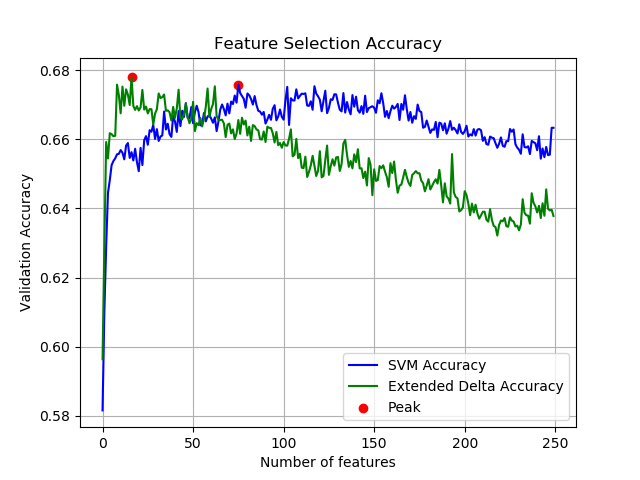
\includegraphics[scale=0.8]{./pictures/experiments/baselines/FeatureSelect.png}
    \caption{The process of the greedy feature selection of the SVM and the Extended Delta Method}
    \label{fig:fs_results}
\end{figure}


\subsection{Hyper Parameter Selection}

As mentioned in the previous section, due to computational time, we were unable
to do the hyper parameter selection parallel with the feature selection. 
For that reason we chose to split it up, selecting our features first, and the 
fine tuning our parameters based on those selected features.

This means that our implementation very closely mimics the one used in the
previous example. On both cases we start out with two lists of possible hyper
parameter values:

\begin{align}
SVM&:
		\begin{array}{lr}
        C=\{10^{-2}, 10^0, 10^2, 10^4, 10^6, 10^8, 10^{10}\}\\
        \gamma=\{10^{-7}, 10^{-5}, 10^{-3}, 10^{-1}, 10^{1}, 10^3, 10^5\}
        \end{array}\\
\text{Extended Delta}&:
		\begin{array}{lr}
        p=\{1,2,3,4,5\}\\
        K=\{1,2,3,4,5,6,7,8,9,10,11,12,13,14,15\}
        \end{array}
\end{align}

The one parameter yet to be explained i $p$, which refers to the p in the
minkowski distance.

$$
D(X,Y) = \left(\sum_{i = 1}^n |x_i - y_i|^p\right)^{1/p}
$$

Where $p=1$ and $p=2$ is the manhattan and eucledian distance respective.

We perform a grid search over all these parameters. For each variation of the
hyper parameters we average the performance of the method over all unique
authors in the training set, in a manner very similar to the feature selection.
A key difference is that rather than using 3 fold cross validation, we now use
leave one out cross validation. We aren't performing nearly as many iterations
this time around, which is why this change was made. In this case, we loop
over all unique authors one time for each combination of hyper parameter, the
number of which dwarfs the amount in the feature selection. The accuracy of each
parameter configuration can be seen in Figure TODO:ref, and Figure TODO: ref.

After the best parameters were found, we apply the methods to the 20\% we set
aside for validation originally. This resulted in the SVM getting an accuracy of
0.713 with its best parameters being $C=100.0$ and $\gamma=1000$.

TODO: Extended Delta Results

%TODO: Try using all features.


\subsection{Deep Learning}

The main attraction of our authorship verification task, is the implementation
and testing of different \gls{NN}. In the following sections we will go through
the different iterations of networks we have produced. A glossary of the
different layers used can be seen in Figure \ref{glossary}. Throughout out
experiments, we used a 0.5 threshold for classification.

\begin{landscape}
    \begin{table}
        \centering
        \caption{Glossary used when performing experiments, and creating their
            associated models.\cite{chollet2015keras}}
        \label{glossary}
        \begin{tabular}{|L{3cm}|L{9cm}|L{11cm}|}
            \hline
            % TODO: Should center header.
            \textbf{Layer}                                                     &
            \textbf{Description}                                               &
            \textbf{Actively Used Parameters}                                 \\
            \hline

            Input                                                              &
            Serves as the entrypoint of the network, by receiving a set of
            texts and feeding it trough the network.                           &
            \begin{minipage}[t]{\linewidth}
            \begin{compactdesc}
                \item[Shape] The dimensions of each sample give to the input.
            \end{compactdesc}
            \end{minipage}                                                    \\
            \hline

            Embedding                                                          &
            Taking in an encoded sample, it produces a dense vector
            representation for each different. More details can be found in
            Section \ref{subsubsec:layers}.                                    &
            \begin{minipage}[t]{\linewidth}
            \begin{compactdesc}
                \item[Input Dim] Size of vocabulary.
                \item[Output Dim] Size of vector used to represent embedding.
            \end{compactdesc}
            \end{minipage}                                                    \\
            \hline

            Convolutional                                                      &
            Applies convolution to the data it recieves according to the
            decription, found in Section \ref{subsubsec:layers}.               &
            \begin{minipage}[t]{\linewidth}
            \begin{compactdesc}
                \item[Filters] Dimensionality of the output, ie. number of
                    filter from the convolution.
                \item[Kernel Size] Integer or list describing size of
                    convolution window.
                \item[Strides] Stride length of the convolutional window.
                \item[Activation] The activation function to be applied after
                    the convolution.
            \end{compactdesc}
            \end{minipage}                                                    \\
            \hline

            Global Max Pooling                                                 &
            Extracts the maximum value from each of the provided data          &
            No parameters.                                                    \\
            \hline

            Concatenation                                                      &
            As the name suggests, this layers simply concatenates the data it
            receives from different layers                                     &
            No parameters.                                                    \\
            \hline

            Merge                                                              &
            Merges its inputs, using a specified function to generate a single
            output.                                                            &
            \begin{minipage}[t]{\linewidth}
            \begin{compactdesc}
                \item[Function] The function used to merge the recieved data.
            \end{compactdesc}
            \end{minipage}                                                    \\
            \hline

            Dense                                                              &
            A simple fully connected layer, taking in data and applying the
            function described in Section \ref{sec:neurons}.                   &
            \begin{minipage}[t]{\linewidth}
            \begin{compactdesc}
                \item[Units] Number of neurons in in the layer.
                \item[Activation] The activation function to be applied.
            \end{compactdesc}
            \end{minipage}                                                    \\
            \hline

            Dropout                                                            &
            Drops a fraction it receives, with the goal of preventing
            overfitting.                                                       &
            \begin{minipage}[t]{\linewidth}
            \begin{compactdesc}
                \item[Rate] The fraction of data it receives dropped.
            \end{compactdesc}
            \end{minipage}                                                    \\
            \hline

            Lambda                                                             &
            Applies a specified function to the input it receives              &
            \begin{minipage}[t]{\linewidth}
            \begin{compactdesc}
                \item[Function] The function applied.
            \end{compactdesc}
            \end{minipage}                                                    \\
            \hline

            Reshape                                                            &
            Reshapes the data it receives.                                     &
            \begin{minipage}[t]{\linewidth}
            \begin{compactdesc}
                \item[Dim] Dimensionality to reshape to.
            \end{compactdesc}
            \end{minipage}                                                    \\
            \hline

            GRU                                                                &
            A gated recurrent unit is applied to the data according to the
            description found in Section \ref{subsubsec:layers}.               &
            \begin{minipage}[t]{\linewidth}
            \begin{compactdesc}
                \item[Unit] Number of neurons in the layer.
            \end{compactdesc}
            \end{minipage}                                                    \\
            \hline

            LSTM                                                               &
            A Long Short-Term Memory layer, which works according to the
            description in Section \ref{subsubsec:layers} is applied to the
            given data.                                                        &
            \begin{minipage}[t]{\linewidth}
            \begin{compactdesc}
                \item[Unit] Number of neurons in the layer.
            \end{compactdesc}
            \end{minipage}                                                    \\
            \hline
        \end{tabular}
    \end{table}
\end{landscape}

\subsubsection{Siamese Neural Network - Iteration 1}

The network we used to try and solve the problem is shown in Figure
\ref{fig:network_1}. The Siamese part of the network is the Convolutional
Layer. We used 1000 filters of size 10. That means that 1000 different features
are supposed to be learned by the network and each feature can use a local
context of 10 characters to extract a feature. After the convolution we have a
max-over-time pooling layer. The layer takes the maximum value of each feature
such that we have 1000 features from each text. We then have a normal dense
neural network on top of that which are given the features of both texts. The
dense network is then supposed to learn how to compare the features from the two
texts. We have 1 dense hidden layer each with 500 neurons. At the end we have
a output layer with two outputs. The activation function for all layers except
the last one is the rectified linear unit and the activation function of the
last layer is the softmax function. The output of the network is a probability
distribution over the two classes.

The input to the network first goes through an embedding layer. The embedding
layer transforms integers into dense vectors of floating point numbers. The
embedding layer functions as a lookup table such that each integer is mapped
to the same dense vector. The embedding is trainable meaning that better
embeddings will be learned while the network is training.

\begin{figure}[htb]
    \centering
    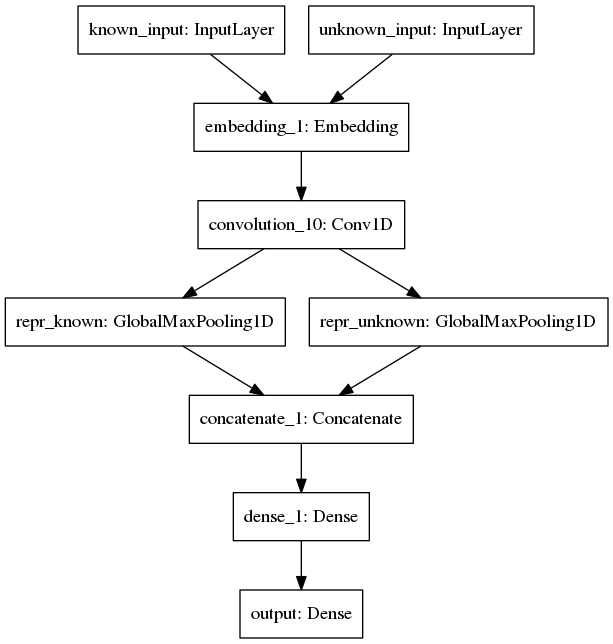
\includegraphics[width=0.6\textwidth]{./pictures/experiments/network1.png}
    \caption{Illustrate the structure of our first Siamese Neural Network
        Architecture.}
    \label{fig:network_1}
\end{figure}

The network obtained a validation accuracy of 0.68684. We have shown both the
training and validation accuracies in the different epochs in Figure
\ref{fig:network1_accuracies}. In that plot we can see that the network very
quickly overfits the training data and no longer learns anything general.

\begin{figure}[htb]
    \centering
    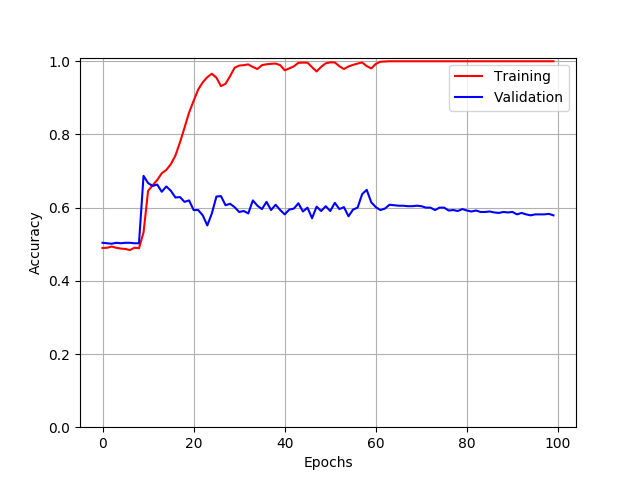
\includegraphics[width=0.5\textwidth]{./pictures/experiments/network_1_accuracies.png}
    \caption{Training and validation accuracies for the iteration 1 network in
        the different epochs of the networks execution.}
    \label{fig:network1_accuracies}
\end{figure}


\subsubsection{Siamese Neural Network - Iteration 2}

% TODO: Illustrate how dropout corresponds to training different subnetworks in
% each iteration.

In our last network we observed that the network after a few number of epochs
overfitted on the training dataset. The validation accuracy quickly began
stalling as the training accuracy went to 100\%. We therefore focused our
second network architecture on limiting overfitting. We added a dropout layer
before the output layer. The layer prevents overfitting by making sure that
the network cannot rely on the output of all neurons during training. This
unpredictability makes it harder for the network to learn specific quirks of
the training dataset since small quirks will only be picked up by a small
amount of neurons while larger trends will be represented by a larger set
of neurons. \cite{JMLR:v15:srivastava14a} investigated the use of dropout
layers in different problem settings. They found that dropout layers reduced
overfitting in all problems they looked at. In particular they found that
document classification which is similar to what we are doing were also
improved. The main drawback of a dropout layer is that it increase the run time
of training the networks (\cite{JMLR:v15:srivastava14a}).

In iteration 1 the function we used to merge features from the known and unknown
text together were a concatenation. If we let the extracted features of the
known text be $K_i$ and the extracted features of the unknown text be $U_i$ then
$K_0$ and $U_0$ correspond to the same feature extracted from the two texts. The
concatenation merge function would then produce,

\begin{equation}
    merge(K, U) \rightarrow \left(
        K_0, K_1, \dots, K_n, U_0, U_1, \dots, U_n
    \right)^T.
\end{equation}

That means that the neural network would have to figure out by itself that input
$0$ were related in particular to input $n + 1$. To save the network that task
we also replaced the merging function to the absolute difference of the feature
vectors. That means that our merge function became,

\begin{equation}
    merge(K, U) \rightarrow \left(
        (|K_0 - U_0|), (|K_1 - U_1|), \dots, (|K_n - U_n|)
    \right)^T.
\end{equation}

So the network no longer has to learn arbitrary indexes. Instead it can learn
which features is important for authorship verification and learn thresholds for
when each feature is important. With the new merging we will have a large number
whenever the two features are far apart and a small number whenever they are
close to each other.

We changed the convolutional filters we used from 1000 convolutional filters of
size 10 to 500 convolutional filters of size 4 and 500 convolutional filters of
size 8. The idea was that the filters could learn different features where some
of the features would consist of a large number of characters and other of the
features would consist of a small number of characters. The architecture of our
network from iteration 2 is shown in Figure \ref{fig:network_2}.

\begin{figure}
    \centering
    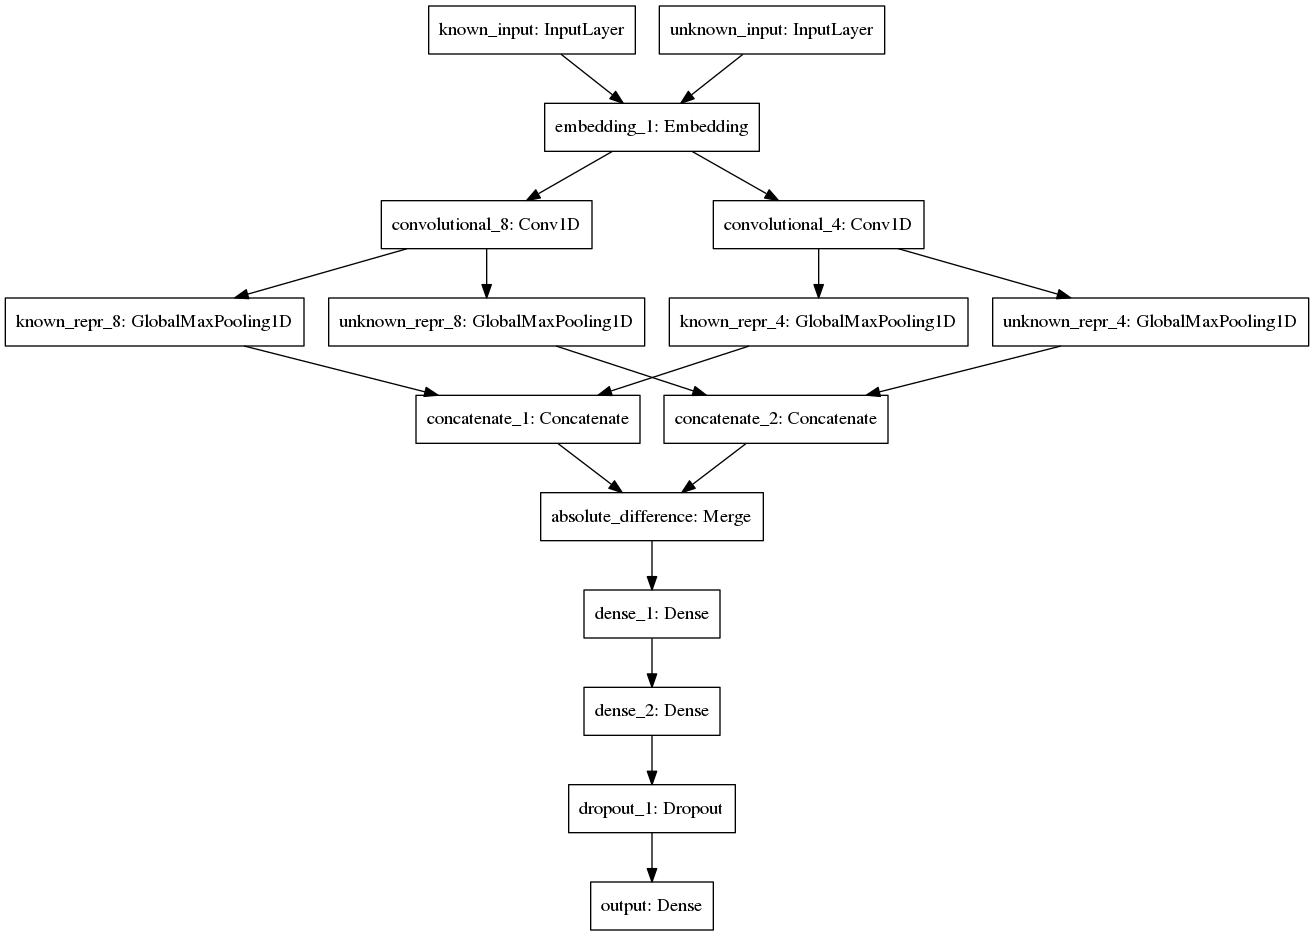
\includegraphics[width=\textwidth]{./pictures/experiments/network2.png}
    \caption{Illustrate the structure of our second Siamese Neural Network
        Architecture.}
    \label{fig:network_2}
\end{figure}

We also added more dense layers to the model. A plot of the
training and validation accuracies per epoch can be seen in Figure
\ref{fig:network2_accuracies}.

\begin{figure}
    \centering
    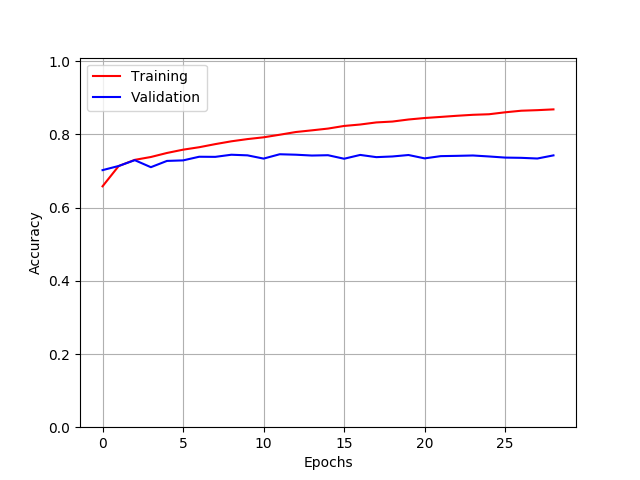
\includegraphics[width=0.5\textwidth]{./pictures/experiments/network_2_accuracies.png}
    \caption{Shows the training and validation accuracies on the second
        network.}
    \label{fig:network2_accuracies}
\end{figure}

The maximum validation accuracy obtained were 0.74464 in epoch 12.


\subsubsection{Siamese Neural Network - Iteration 3}

In iteration 2 we observed that the network seemed to learn everything in the
first epoch and didn't improve much after that. We also observed that the
accuracy improved compared to the first network. We therefore wanted to try a
larger network which would be able to hopefully learn more and obtain a higher
accuracy than our first two networks.

We both tried adding more convolutions and adding more dense layers. Our third
network use 700 convolutions of size 8 (currently drawn confusingly) and 500
convolutions of size 4. The network then contains 4 dense layers all with 500
hidden neurons with \gls{ReLu} activation function. Then a dropout layer with
30\% dropout and finally the output layer with 2 neurons and a softmax
activation function. The function we use to combine the features from the two
texts are still the absolute difference as that seemed to work fine for the
previous network. We have shown the structure of the third network in Figure
\ref{fig:network3}.

\begin{figure}
    \centering
    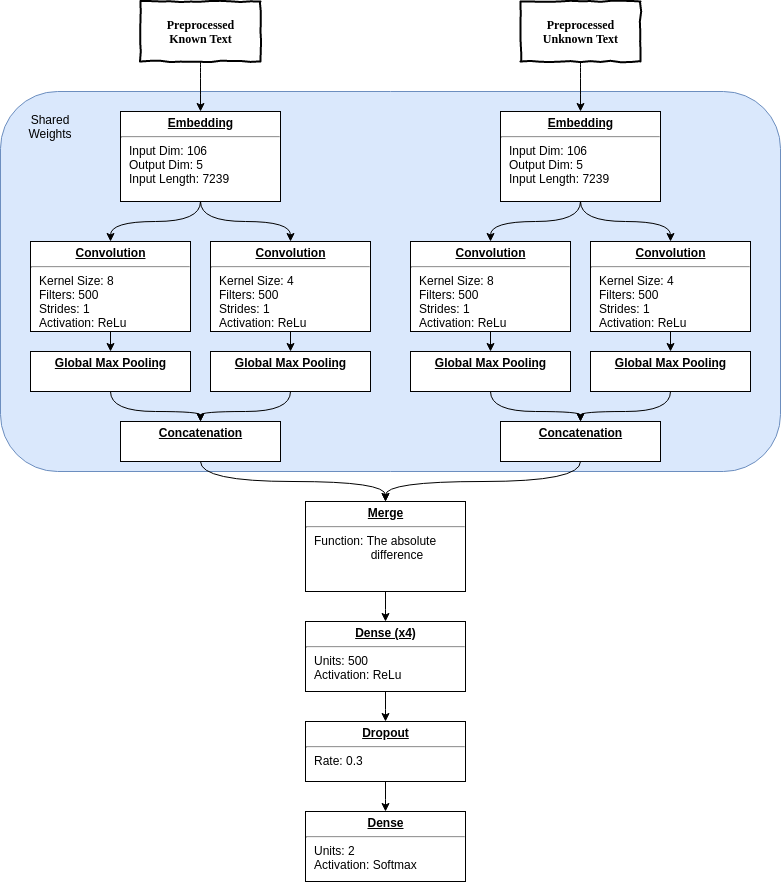
\includegraphics[width=\textwidth]{./pictures/experiments/network3/network3.png}
    \caption{Illustrate the structure of our third Siamese Neural Network.
        Weights are shared by the embedding layers and the convolutional
        layers.}
    \label{fig:network3}
\end{figure}

Our third network were able to obtain an accuracy of 0.83612. We have shown the
training and validation accuracies in Figure \ref{fig:network_3_accuracies}. We
can see that the network quickly improve to about 80\% accuracy and after that
not much happens.

\begin{figure}
    \centering
    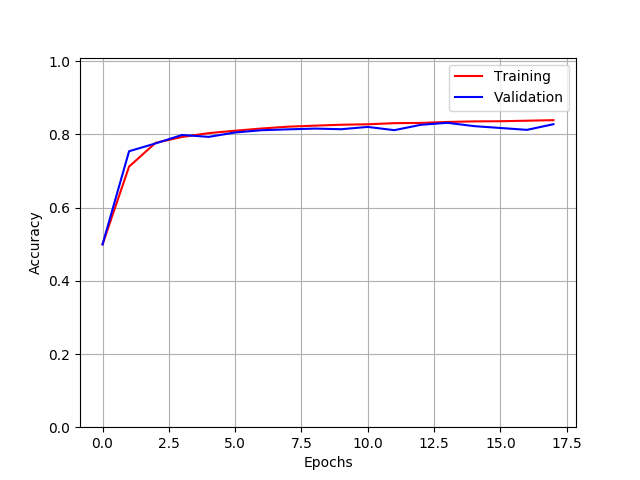
\includegraphics[width=0.5\textwidth]{./pictures/experiments/network_3_accuracies.png}
    \caption{Shows the training and validation accuracies over the epochs of
        training on the third network.}
    \label{fig:network_3_accuracies}
\end{figure}

To get an idea of which features the network were looking at we looked at the
output of the convolutional layers. After the convolutional layers we have a
max-over-time pool so we know that higher values are important. We could then
take a text, feed it to the network, find the index of the maximum output of
the convolutional layers and then show the text snipped (char-N-gram) that
produced that high value. We then did that for all the texts in the dataset. The
first filter in the network for example yielded many short strings ending with 3
newlines. Some examples of these are,

\begin{lstlisting}[gobble=4]
    'adsen\n\n\n'
    'ndsen\n\n\n'
    'umeer\n\n\n'
    'endte\n\n\n'
    'ingen\n\n\n'
    'ehren\n\n\n'
    'elsen\n\n\n'
    'ommer\n\n\n'
    'Ruter\n\n\n'
    'ummer\n\n\n'
    'ersen\n\n\n'
    'ansen\n\n\n'
    'heden\n\n\n'
    'ensen\n\n\n'
    'arsen\n\n\n'
    'orten\n\n\n'
    'ulsen\n\n\n'
    'orgen\n\n\n'
\end{lstlisting}

Many of those short string looks like the ending of common Danish
names followed by three newlines. Here are some examples of the
names taken from a list of the 100 most frequent surnames in Denmark
\footnote{http://www.mydanishroots.com/surnames-meaning-and-origin/the-100-most-
common-surnames-in-denmark.html},

\begin{description}
    \item[adsen:] Madsen.
    \item[ndsen:] Svendsen, Frandsen.
    \item[elsen:] Nielsen, Mikkelsen.
    \item[ersen:] Pedersen, Andersen, Petersen, Iversen, Jespersen.
    \item[ansen:] Hansen, Christiansen, Johansen, Kristiansen.
    \item[ensen:] Jensen, Christensen, S\o rensen, J\o rgensen, Kristensen,
        Mortensen, Mogensen.
    \item[arsen:] Larsen.
    \item[ulsen:] Poulsen.
\end{description}

The network therefore seems to have learned that a name followed by whitespace
are an important feature when determining the authorship of a text. Clearly when
a student buy an assignment from a ghost writer the text will contain the
students own name. Therefore these features are counter productive since the
network learns that as a result of how we have created the training dataset
where each text has the correct authors name in it.


\subsubsection{Siamese Neural Network - Iteration 4}

In this iteration we trained the third network again but now using a dataset
where names were substituted by empty strings. We wanted to see how well the
network would perform when it was not able to use peoples names as a feature.
A graph of the training and validation accuracies can be seen in Figure
\ref{fig:network_4_accuracies}. The best validation result we found was in epoch
22 with an accuracy of 0.79843. That means that we lost about 4\% accuracy now
that we can no longer look at peoples names.

\begin{figure}
    \centering
    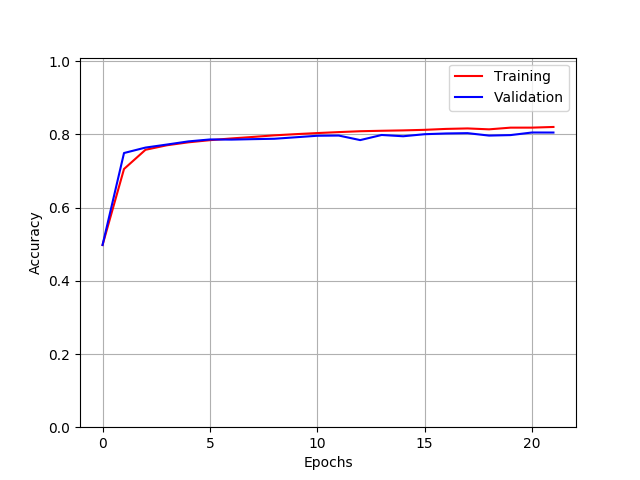
\includegraphics[width=0.5\textwidth]{./pictures/experiments/network_4_accuracies.png}
    \caption{Shows the training and validation accuracies over the epochs of
        training on the fourth iteration of the network.}
    \label{fig:network_4_accuracies}
\end{figure}

We wanted to verify whether or not the network still looked at the names of the
authors. It is not possible for us to look at all 1200 filters but we looked
at a couple and did not find any that looked like they were looking at names.
However we did find that the network now seems to be looking at which class
the student is in. The classes in Danish schools are typically written as 1.p,
1.q, 2.p, 2,q, etc. and we found that one of the convolutional 4 filters were
looking at character sequences such as those. We have generated a couple of
tables that shows what the network is now looking at. We generated the tables by
taking the first 50 texts from the dataset and extracting the maximum value of a
particular filter from each text. That gives a single string of the convolution
size from each text and a number which is higher the more important that string
is. We then sorted the extractions by the importance score. The result of a
couple of the filters are shown in Figures \ref{fig:features_convolution_8_1},
\ref{fig:features_convolution_8_5}, \ref{fig:features_convolution_8_100} and
\ref{fig:features_convolution_4_100}. The first figure looks at whether or not
authors use the phrase "s\aa\ at" (such that). Inexperienced Danish writers will
often use the phrase which is considered grammatically incorrect in most Danish
sentences. Therefore the network seems to have learned that some writers use
"s\aa\ at" while others don't and that it is an important phrase when verifying
authorship. The second figure seems to look at whether or not an authors uses
the phrase "meget" (most). Some authors apparently often describe things using
"meget" while others do not. The third figure shows that the network looks at
which authors use the phrase "at de" or "at der" ("that they" or "that there").
The fourth filter is the one that seems to look at which class a student is in.
In our constructed dataset the class of a student will always be a good feature
since we don't have any actual ghost writers. However a ghost writer would write
the correct class of the student on their submission. Therefore we don't want
the network to learn that particular feature.

Our main problem is that the networks keep using metadata from the texts to
make the predictions. The metadata will always match even though a ghost writer
has written the assignment. It is probably not possible for us to remove all
metadata from all texts. Even though names are supposed to have been removed
the dataset still contains a couple of them and there is so many different ways
of writing the class of a student that it is not feasible for us to remove
all of them. The metadata will typically occur in the beginning of the text
and sometimes throughout the text in headers. When training a neural network
on images it is normal practice to rotate, shift, shear and zoom the images
randomly during training. The shifting of the images produces new images where
part of the image is no longer part of the training set. In each epoch the
image is shifted a different amount in different directions and the network can
therefore learn to recognise objects even though part of the image is not there.
We wanted to do something similar for the texts we are training on. At the
moment the network relies on finding metadata in the text. That is only possible
when it is given the whole text since metadata will only occur in parts of the
text. We therefore want to try to only give part of the texts to the network
during training. We can do that by replacing some random part of the input text
with a special value during training. For example each time a text is used
during training we might replace 50\% of it with a special garbage character.
Therefore the network will no longer be able to rely on finding metadata about
the text since the metadata will not always be present.

Another problem our current networks has is that each filter extract
only a single value from a text. For example the filter shown in Figure
\ref{fig:features_convolution_8_1} that looked at the phrase "s\aa\ at". The
filter is able to find out whether or not a text contains the phrase but are not
able to say anything about how often that phrase is used by the author. To find
out how often a phrase is used we need to stop using max over time pooling and
start using some kind of average.


\subsubsection{Siamese Neural Network - Iteration 5}

The problems in the previous network were mainly due to the use of a global
max pool. That allowed our networks to look at the presence of certain strings
in texts. Our fifth iteration therefore does not include any global max pools.
Furthermore the network is an \gls{RNN}. We used an \gls{RNN} since they are
very good at sequence processing \cite{DBLP:series/sci/2012-385}. A text can
be viewed as a sequence where each character is a different timestep in the
sequence. We took inspiration from \cite{DBLP:journals/corr/RuderGB16c} who
used an \gls{RNN} for authorship verification. However instead of representing
the text as a sequence of sentences we represent it as a sequence of characters
and instead of using the output of each timestep we only used the last output
of the \gls{RNN}. We used the same basic architecture as before. Two texts are
presented to the network at the same time and features are extracted from the
texts by a Siamese Network. The features are then compared using a normal dense
network. In this iteration we used a combination of convolutions and \gls{RNN}'s
to extract the features. The input is as usual encoded in an embedding layer.
The embedding layer is followed by a convolutional layer of size 8 and stride
1. The idea is that the convolutional layer can look at 8 characters at a time
and learn features from that. After the convolutional layer we have a max pool
with pool size 8. That is mainly to save computation power as the size of the
texts are reduced to $\frac{1}{8}$ of the original size. After the max pool we
have a \gls{LSTM} layer with 100 output neurons. The \gls{LSTM} layer loops
through the output from the convolution and max pool and extracts 100 features
from it. Now we have 100 features from each of the input texts. As earlier we
combine the features with the elementwise absolute difference. On top of that
Siamese part of the network we compare the features extracted with a classic
dense network. The network has a single layer with 500 neurons and activated by
the \gls{ReLu} activation function. Lastly we have a dropout layer with 30\%
dropout and the output layer with a softmax as before. We have shown the network
in Figure \ref{fig:network5}.

\begin{figure}
    \centering
    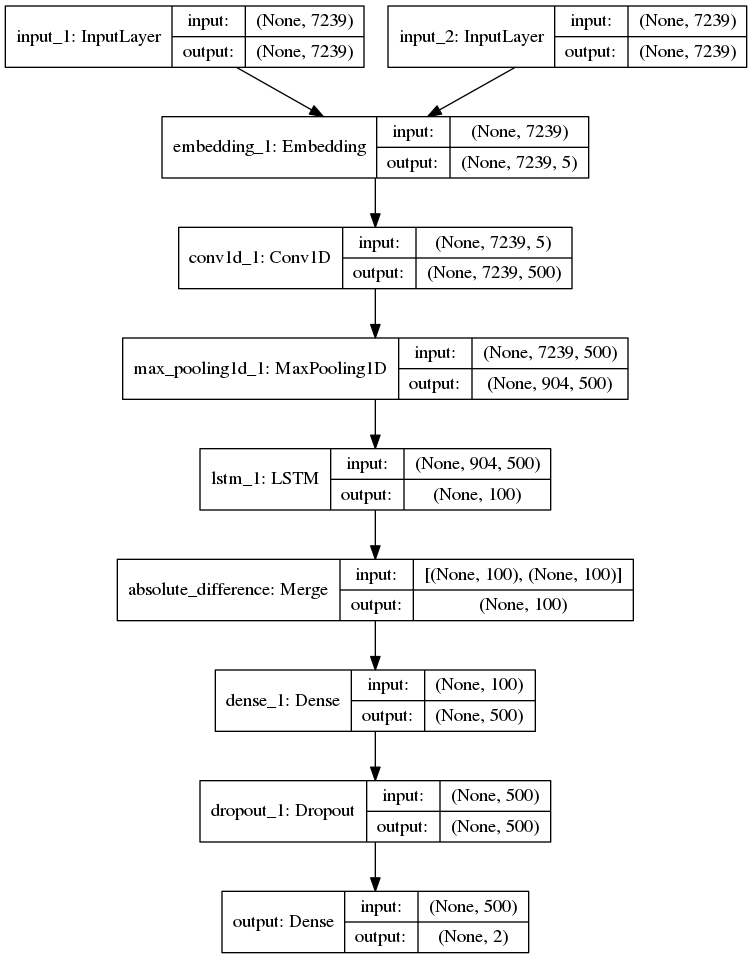
\includegraphics[width=\textwidth]{./pictures/experiments/network5.png}
    \caption{Illustrate the structure of our fifth Siamese Neural Network.
        Weights are shared by the embedding layers, the convolutional layer and
        the LSTM layer. This Figure will be replaced by the new format when we
        decide what that format is.}
    \label{fig:network5}
\end{figure}

The network reached an accuracy of 0.89393 in epoch 18. The training and
validation accuracies are shown in Figure \ref{fig:network_5_accuracies}. At the
end of the training the network suddenly goes from about 90\% accuracy and back
to 50\% accuracy. A reason for that happening could be that the optimizer
overshot a target and therefore ended up with a worse result.

\begin{figure}
    \centering
    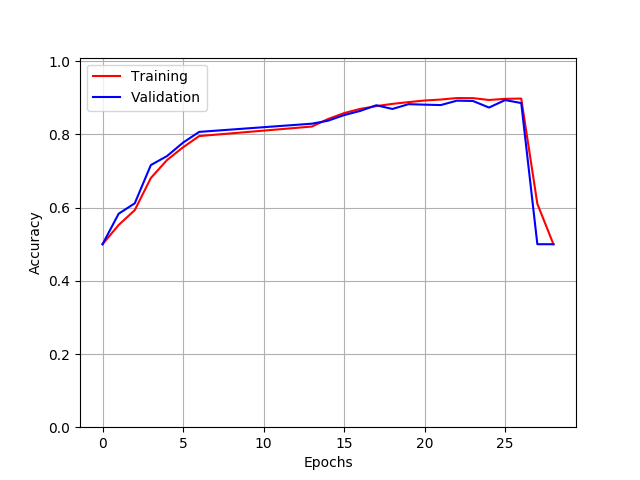
\includegraphics[width=0.5\textwidth]{./pictures/experiments/network_5_accuracies.png}
    \caption{Shows the training and validation accuracies over the epochs of
        training on the fifth iteration of our networks.}
    \label{fig:network_5_accuracies}
\end{figure}

The students normally write their personal information in the beginning of
assignments. Earlier we described that MaCom removed most of the names from
the assignment. But they still contain information such as classes, dates and
a different number of new line characters per student. We were suspicious
that the networks still made use of some meta data from the texts so we tried
training the network again but where we removed the 200 first characters from
each text. Since most of the metadata are located in the beginning of the
text we hoped that that would remove the problem. On this new dataset the
best validation accuracy was obtained in epoch 3 with an accuracy of 0.53233.
Clearly the network relied exclusively on the metadata in the beginning of
the texts. We have shown the training and validation accuracies in Figure
\ref{fig:network_5_accuracies_2}.

\begin{figure}
    \centering
    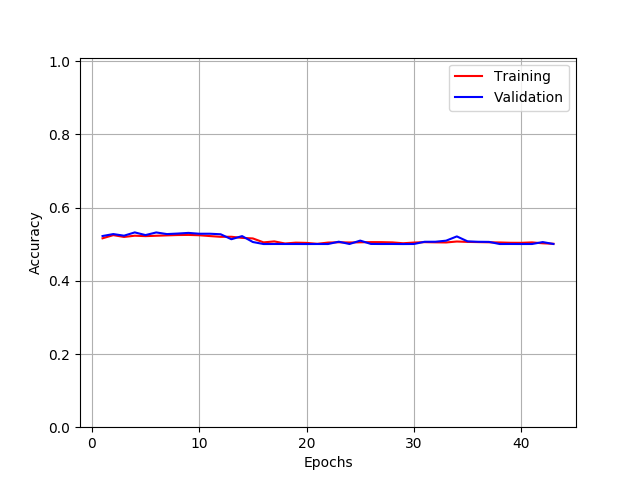
\includegraphics[width=0.5\textwidth]{./pictures/experiments/network_5_accuracies_2.png}
    \caption{Shows the training and validation accuracies over the epochs of
        training on the fifth iteration of our networks where we removed the 200
        first characters.}
    \label{fig:network_5_accuracies_2}
\end{figure}


\subsubsection{Siamese Neural Network - Iteration 6}
\label{subsubsec:siamese_neuraon_network_iteration_6}

In this iteration we trained our third network again but this time with the 200
first characters removed like in Iteration 5. We wanted to see how much worse
the network would perform now that we had hopefully removed some more personal
information from what the network had available to look at. We have shown the
training and validation accuracies in Figure \ref{fig:network_6_accuracies}. The
best validation accuracy was obtained in epoch 57 with an accuracy of 0.74370.
That means that we lost about 5\% accuracy by removing the first 200 characters.

\begin{figure}
    \centering
    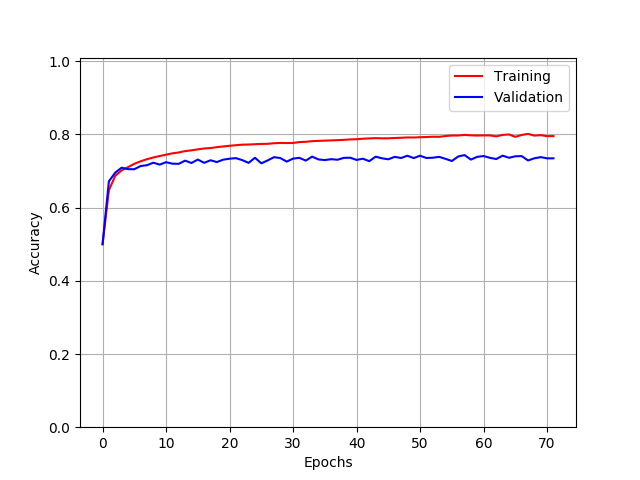
\includegraphics[width=0.5\textwidth]{./pictures/experiments/network_6_accuracies.png}
    \caption{Shows the training and validation accuracies over the epochs of
        training on the sixth iteration of our networks.}
    \label{fig:network_6_accuracies}
\end{figure}


\subsection{Prediction System}

Our prediction system has several hyperparameters we have to choose to get
the best results. We recall that MaCom wanted a system that had an accusation
error of less than 10\%. We can use the threshold parameter $\theta$ in the
prediction system to control how many people we accuse. The best parameters
for the prediction system is those parameters that gives the highest accuracy
subject to the constraint that the accusation error should be less than 10\%.
To tune the parameters we use a validation dataset $V$ consisting of a set of
tuples $(\alpha, t_u)$ where $\alpha$ is a candidate author and $t_u$ is a text
of unknown authorship. None of the authors in $V$ has been seen by the networks
during training and none of the texts $t_u$ has been seen by the networks during
training. The parameters that maximize the accuracy subject to the bounded
accusation error is the same as the parameters that minimize the error rate
subject to the bounded accusation error. That optimization problem is,

\begin{equation}
    \label{eq:prediction_system_minimization}
    \begin{aligned}
        & \underset{\theta, w}{\text{minimize}}
        & & \sum_{(\alpha, t_u) \in V} \left|
            P(f, w, T_\alpha \setminus \{t_u\}, t_u, \theta) -
            \mathbbm{1}_{T_\alpha}(t_u)
        \right| \\
        & \text{subject to}
        & & \frac{\sum_{(\alpha, t_u) \in V} \mathbbm{1}_{T_\alpha}(t_u) \cdot
            \left(1 - P(f, w, T_\alpha \setminus \{t_u\}, t_u, \theta)\right)}
{\sum_{(\alpha, t_u) \in V} (1 - P(f, w, T_\alpha \setminus \{t_u\}, t_u, \theta)} <
            \frac{1}{10} 
    \end{aligned}
\end{equation}

In the optimization problem we fix the network $f$ we validate. The expression
we minimize is the number of errors made in prediction over the validation set
$V$. Consider a problem $(\alpha, t_u) \in V$ where $t_u \in T_\alpha$. Then we
know that $\mathbbm{1}_{T_\alpha}(t_u) = 1$ from the definition of the indicator
function then if the prediction system returns the correct result 1 we have,

\begin{equation}
    e = \left|
        P(f, w, T_\alpha \setminus \{t_u\}, t_u, \theta) -
        \mathbbm{1}_{T_\alpha}(t_u)
    \right| = |1 - 1| = 0,
\end{equation}

and if the prediction system returns the incorrect result 0 we have,

\begin{equation}
    e = \left|
        P(f, w, T_\alpha \setminus \{t_u\}, t_u, \theta) -
        \mathbbm{1}_{T_\alpha}(t_u)
    \right| = |0 - 1| = 1.
\end{equation}

Similarly for a problem $(\alpha, t_u) \in V$ where $t_u \notin T_\alpha$ we
know that $\mathbbm{1}_{T_\alpha}(t_u) = 0$ from the definition of the indicator
function. Then if the prediction system returns the correct result 0 we have,

\begin{equation}
    e = \left|
        P(f, w, T_\alpha \setminus \{t_u\}, t_u, \theta) -
        \mathbbm{1}_{T_\alpha}(t_u)
    \right| = |0 - 0| = 0,
\end{equation}

and if the prediction system returns the incorrect result 1 we have,

\begin{equation}
    e = \left|
        P(f, w, T_\alpha \setminus \{t_u\}, t_u, \theta) -
        \mathbbm{1}_{T_\alpha}(t_u)
    \right| = |1 - 0| = 1.
\end{equation}

That is the expression we minimize is 0 whenever there is no error and 1
whenever there is an error. So we minimize the number of errors we make. The
subject to expression makes sure that the fraction of false accusations we
make is less than $10\%$ of the accusations we make. The expression should be
read as, 

$$ \frac{\textit{false accusations}}{\textit{total accusations}} <
\frac{1}{10} $$

Consider the numerator of the fraction on the left hand side,

\begin{equation}
    \textit{false accusations} = \sum_{(\alpha, t_u) \in V}
    \mathbbm{1}_{T_\alpha}(t_u) \cdot
    \left(1 - P(f, w, T_\alpha \setminus \{t_u\}, t_u, \theta)\right).
\end{equation}

For a $(\alpha, t_u) \in V$ where $t_u \in T_\alpha$ we have that
$\mathbbm{1}_{T_\alpha}(t_u) = 1$ then if $P$ is correct it returns 1 and we
get,

\begin{equation}
    \mathbbm{1}_{T_\alpha}(t_u) \cdot
    \left(1 - P(f, w, T_\alpha \setminus \{t_u\}, t_u, \theta)\right) =
    1 \cdot (1 - 1) = 0,
\end{equation}

and if $P$ is incorrect and returns 0 we have,

\begin{equation}
    \mathbbm{1}_{T_\alpha}(t_u) \cdot
    \left(1 - P(f, w, T_\alpha \setminus \{t_u\}, t_u, \theta)\right) =
    1 \cdot (1 - 0) = 1.
\end{equation}

Similarly for a $(\alpha, t_u) \in V$ where $t_u \in T_\alpha$ we have that
$\mathbbm{1}_{T_\alpha}(t_u) = 0$ and therefore the expression is always
0. Therefore the expression is 1 whenever we have a false accusation and 0
otherwise. The right hand side of the inequality simply counts the number of
accusations by inverting the output of $P$ and divides that by 10. So the
condition makes sure that only 10\% of the accusations we make are false
accusations.

We have chosen to run our prediction system on the network described in Section
\ref{subsubsec:siamese_neuraon_network_iteration_6}. That is the convolutional
neural network using max-over-time pooling after the convolutional layer.
The validation set we run on consists as described only of previously unseen
authors. It consist of 411 different authors and from them we generate two
problems each meaning that we end up with 822 different problems. For each
of the authors we generate a positive sample by taking the newest text as
the unknown text and a negative sample by choosing a random text from some
other author in the set. That is we have a 0.5 split between positive and
negative samples. To find the $\theta$ and $w$ that minimizes equation
\ref{eq:prediction_system_minimization} we cross validate with $\theta \in
0, 0.1, \dots, 1.0$ and $w \in 0, 0.1, \dots, 1.0$ (when $w = 0$ the weights
are uniform). The results of that cross validation are shown in Figure
\ref{fig:prediction_system_results_1}. The $\theta$ and $w$ that gave the best
accuracy while adhering to the constraint was $\theta = 0.2$ and $w = 0.3$ which
had an accuracy of $0.67153$ and an accusation error of $0.09714$.

\begin{figure}
    \centering
    \textbf{Prediction System Results for 0.5 Split}\par\medskip
    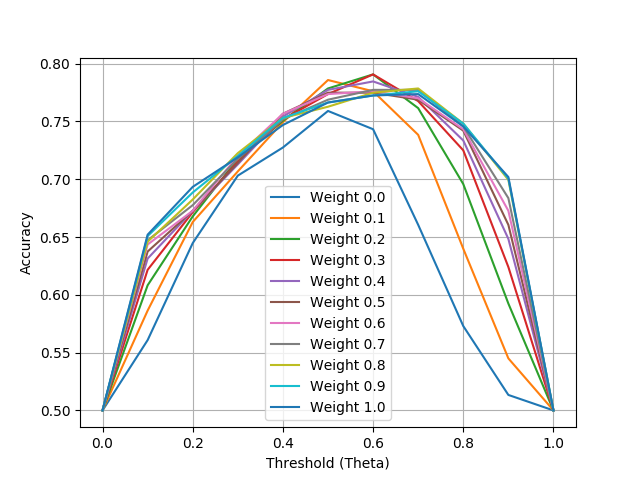
\includegraphics[width=0.49\textwidth]{./pictures/experiments/network3_prediction_system_accuracies.png}
    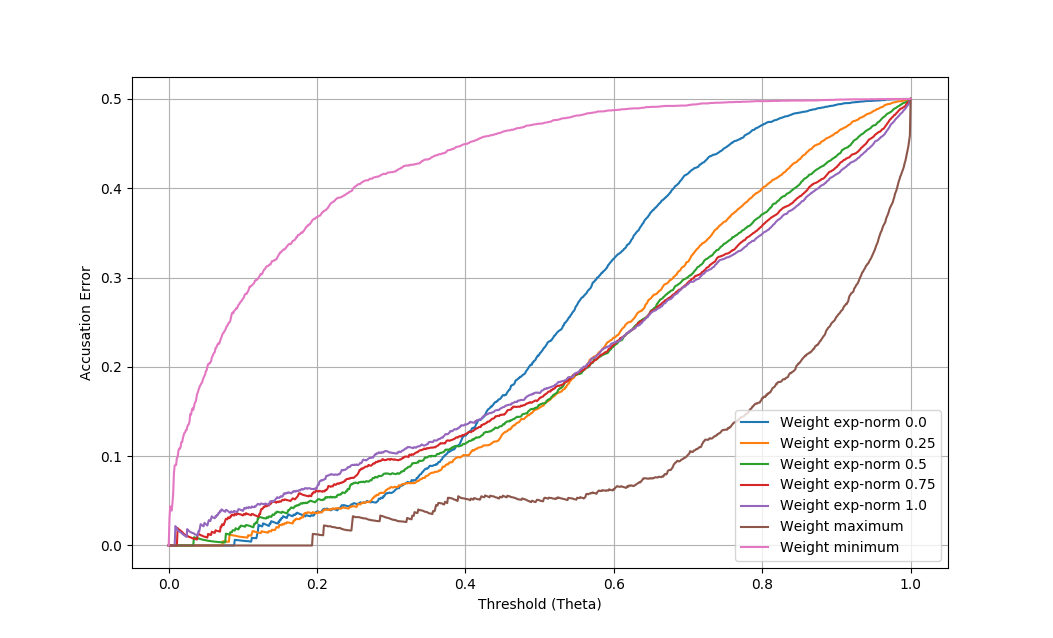
\includegraphics[width=0.49\textwidth]{./pictures/experiments/network3_prediction_system_accusation_error.png}
    \caption{Results of running the prediction system with our best
        convolutional network on a validation dataset with 50\% positive samples
        and 50\% negative samples. In the left graph we show the accuracies
        obtained as a function of $\theta$. There is one line for each weight.
        We can see that as expected the worst weight function are the uniform
        weights. On the right we have shown the accusation error as a function
        $\theta$ again with one line for each weight. We can see that as the
        threshold increases and we accuse more people of cheating the accusation
        error rises.}
    \label{fig:prediction_system_results_1}
\end{figure}

We also tried our prediction system on another validation
set. In the real world it has been estimated that 4\% of
turn ins for the \gls{SRP} are written by "ghost writers"
\footnote{https://politiken.dk/indland/uddannelse/art5603163/Gymnasieelever-\%C2
\% BBSnyderi-beviser-hvor-vanvittig-betydningsfuld-SRP-er-blevet\%C2\%AB}. We
therefore also wanted to find $\theta$ and $w$ for a validation set with only
4\% negative samples instead of 50\% negative samples. We generated 411 positive
samples as before and then for each sample we added a negative sample with a
4\% chance. We ended up with a validation set with 411 positive samples and 16
negative samples. The $\theta$ and $w$ that gave the best accuracy while still
fulfilling the constraint were $\theta = 0.1$ and $w = 0.0$ with an accuracy of
0.97189 and an accusation error of 0.0. With that configuration we caught
$\frac{4}{16}$ of the cheaters with 0 false accusations. We have shown the cross
validation results in Figure \ref{fig:prediction_system_results_2}.

\begin{figure}
    \centering
    \textbf{Prediction System Results for 0.04 Split}\par\medskip
    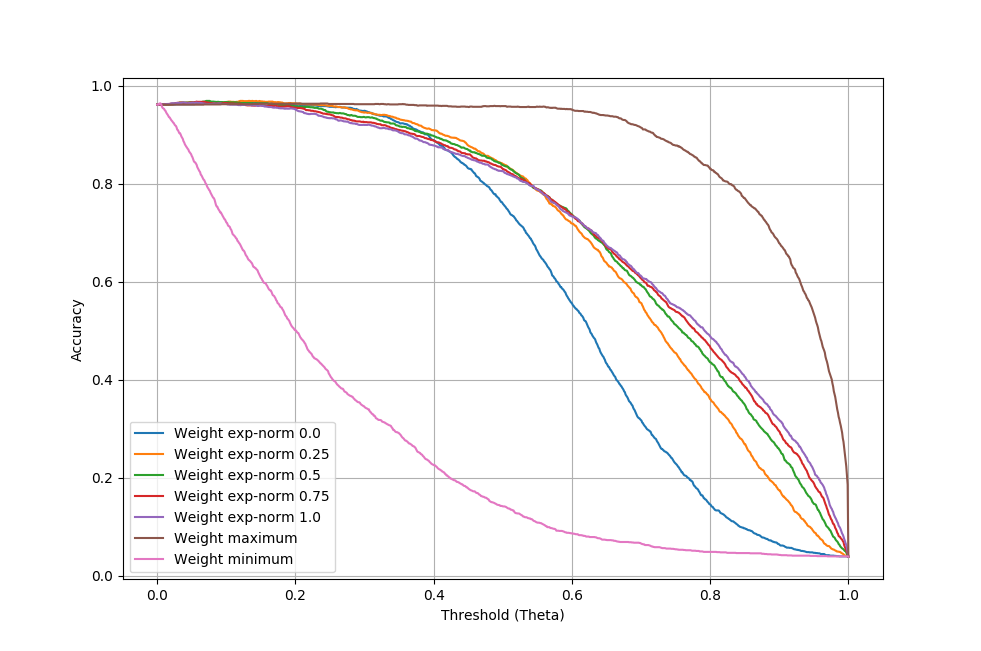
\includegraphics[width=0.49\textwidth]{./pictures/experiments/network3_prediction_system_accuracies_4_percent.png}
    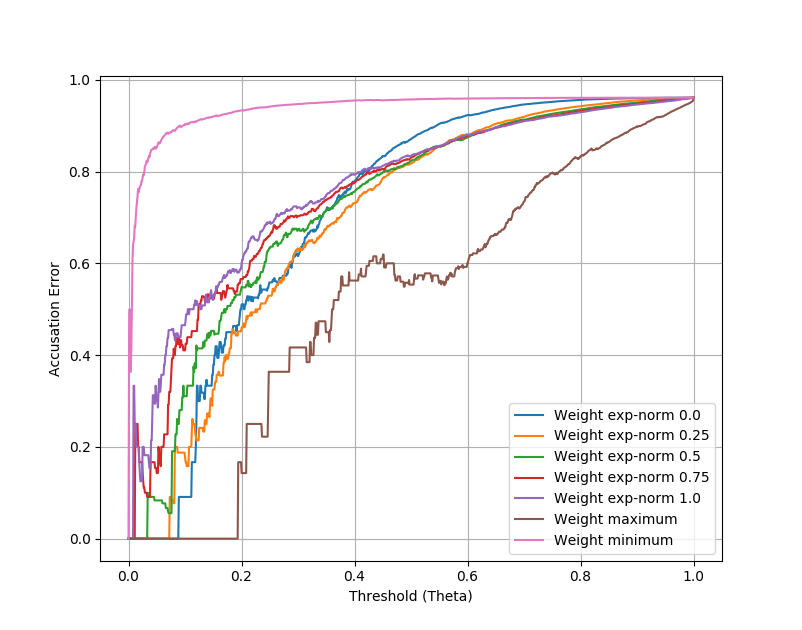
\includegraphics[width=0.49\textwidth]{./pictures/experiments/network3_prediction_system_accusation_error_4_percent.png}
    \caption{Results of running the prediction system with our best
        convolutional network on a validation dataset with about 96\% positive
        samples and about 4\% negative samples. In the left graph we show the
        accuracies obtained as a function of $\theta$. There is one line for
        each weight. On the right we have shown the accusation error as a
        function $\theta$ again with one line for each weight. We can see that
        as the threshold increases and we accuse more people of cheating the
        accusation error rises.}
    \label{fig:prediction_system_results_2}
\end{figure}


TODO:
\begin{itemize}
    \item Describe Optimizers
    \item Describe Dropout
    \item Describe RNN
    \item Use squared distance as merge function to get larger differences
        between close and far apart.
    \item Try to not use dense network but a distance metric.
\end{itemize}
